\def\i{\item}
\graphicspath{{../pictures/vande30/}}
\chapter{Chương 5}
\section{Góc -- số đo góc}
\subsection{KIẾN THỨC CẦN NHỚ}
\subsubsection{Góc}
\begin{enumerate}[--,leftmargin=*]
	\i Góc là hình gồm hai tia chung gốc. Gốc chung của hai tia là đỉnh của góc, hai tia là hai cạnh của góc.
	\begin{center}
%		\begin{tikzpicture}
%			\draw (0,0) -- (4,0) (0,0) -- (3.5,2);
%			\draw (0,0) node [below] {$O$};
%			\draw (0,0) node [below] {$x$};
%			\draw (3.5,2) node [above] {$y$};
%			\draw [->] (-1,1) -- (-0.2,0.2) (1,3) --(2,0.2) (1,3) -- (2.5,1.8);
%			\draw (-1,1) node[above] {Đỉnh};
%			\draw (1,3) node [above] {Cạnh};
%		\end{tikzpicture}
		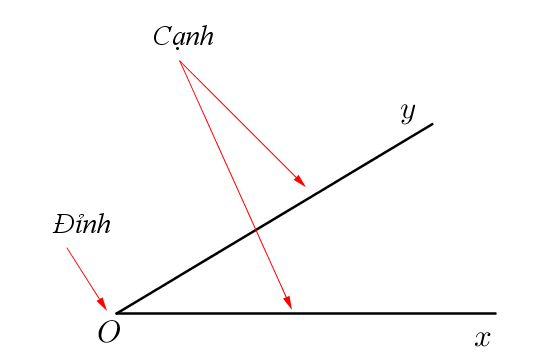
\includegraphics[width= 0.5\linewidth]{vd-30-1}
	\end{center}
	\i Góc  $xOy$, kí hiệu $\widehat{xOy}$ (hay $\widehat{yOx},\,\widehat{O}$) gồm hai tia chung gốc là $Ox$ và $Oy$. Điểm $O$ là đỉnh của góc $xOy$. Hai tia $Ox,\,Oy$ là cạnh của góc $xOy$.
\end{enumerate}
\subsubsection{Điểm trong của góc}
\begin{enumerate}[--,leftmargin=*]
	\immini{\i Ta gọi $A$ là một điểm trong của góc $xOy$
	\i Các điểm nằm trên hai cạnh của góc chẳng hạn như $C$ và các điểm như điểm $B$ không phải là điểm trong của góc $xOy$.}{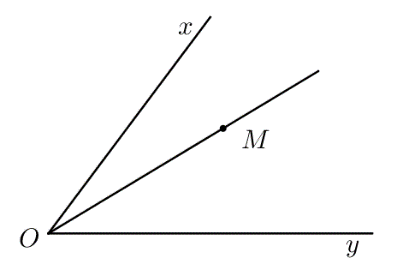
\includegraphics[width= 0.5\linewidth]{vd-30-2}}
\end{enumerate}
\subsubsection{Số đo góc}
\subsubsection*{a. Số đo góc}
\begin{enumerate}[--,leftmargin=*]
	\i Muốn đo góc $xOy$, ta đặt thước đo góc sao cho tâm của thước trùng với $O$, tia $Ox$ đi qua vạch $0$. Khi đó tia $Oy$ đi qua vạch chỉ số đo của góc. Trên hình dưới đây, ta thấy $Oy$ đi qua vạch 110. Vậy góc $xOy$ có số đo là 110 độ. Ta viết $\widehat{xOy}={{110}^\circ}$.\\
	\immini{$\widehat{xOy} = 110^\circ$\\
		(Đọc số ở vòng cung lớn)}{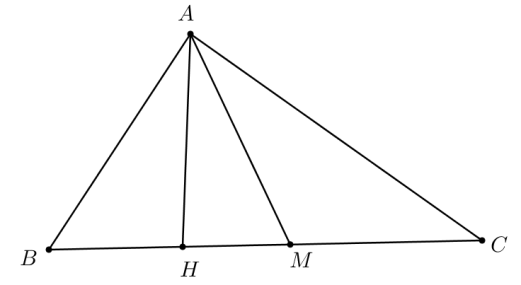
\includegraphics[width= 0.5\linewidth]{vd-30-3}}
	\i Mỗi góc có một số đo. Số đo của một góc không vượt quá ${{180}^\circ}$.
\end{enumerate}
\subsubsection*{b. So sánh góc}
So sánh hai góc bằng cách so sánh số đo của chúng.
\begin{enumerate}[--,leftmargin=*]
	\i Hai góc $\widehat{xAy}$ và $\widehat{vOt}$ có số đo bằng nhau.
	\begin{center}
		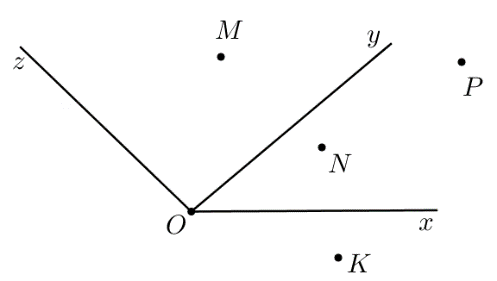
\includegraphics[width= 0.5\linewidth]{vd-30-4}
	\end{center}
	\i Góc $\widehat{tOz}$ có số đo lớn hớn $\widehat{CAB}$, ta viết $\widehat{tOz}>\widehat{CAB}$, ta nói $\widehat{tOz}$ lớn hơn $\widehat{CAB}$.
	\begin{center}
		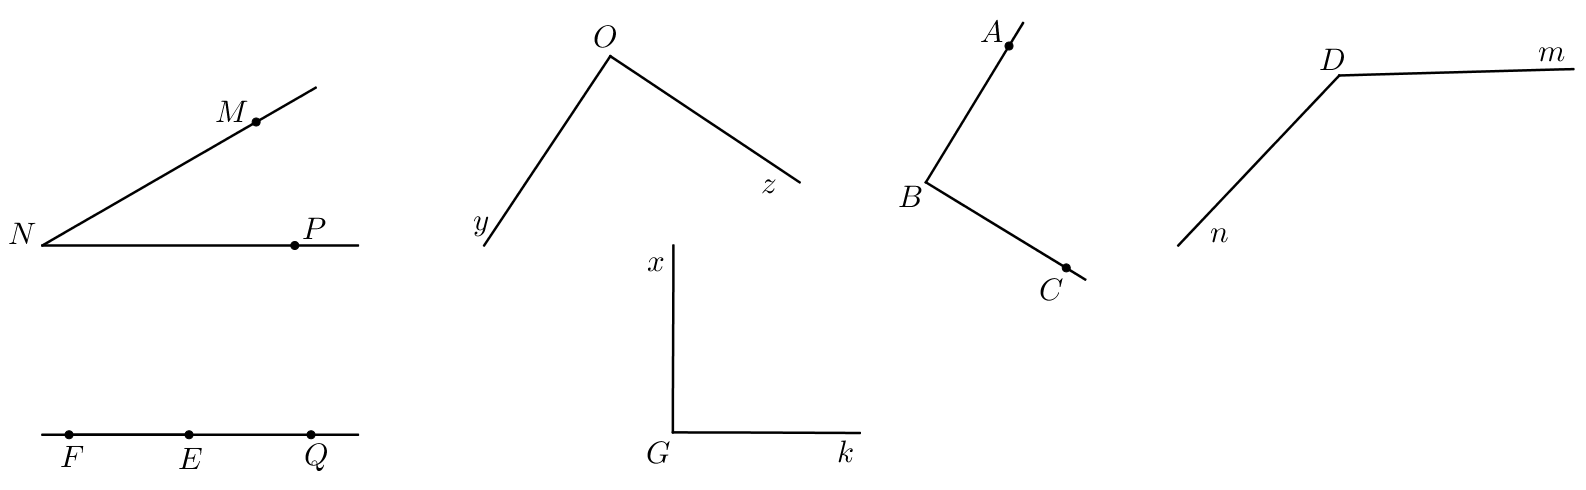
\includegraphics[width= 0.5\linewidth]{vd-30-5}
	\end{center}
\end{enumerate}
\subsubsection*{c. Các góc đặc biệt}
\begin{enumerate}[--,leftmargin=*]
	\i Góc có số đo bằng ${{90}^\circ}$ là góc vuông.
	\i Góc bẹt có số đo bằng ${{180}^\circ}$.
	\i Góc nhỏ hơn góc vuông là góc nhọn.
	\i Góc lớn hơn góc vuông, nhỏ hơn góc bẹt là góc tù.
\end{enumerate}
\subsection{THỰC HÀNH GIẢI TOÁN}
\begin{vd}
	Đọc tên các góc, ghi đỉnh và các cạnh của mỗi góc. 
	\begin{center}
		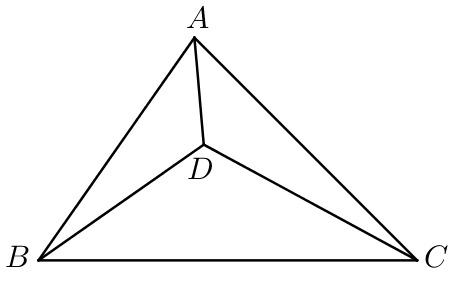
\includegraphics[width= 0.5\linewidth]{vd-30-6}
	\end{center}
	\loigiai{
		\begin{enumerate}[+,leftmargin=*]
			\i Góc $\widehat{xOy}$: đỉnh $O$, cạnh $Ox,Oy$.
			\i Góc $\widehat{vOt}$: đỉnh $O$, cạnh $Ov,Ot$.
		\end{enumerate}
	}
\end{vd}
\begin{vd}
	Xác định các điểm nằm trong góc $\widehat{mOn}$ và các điểm không nằm trong góc $\widehat{mOn}$.
	\begin{center}
		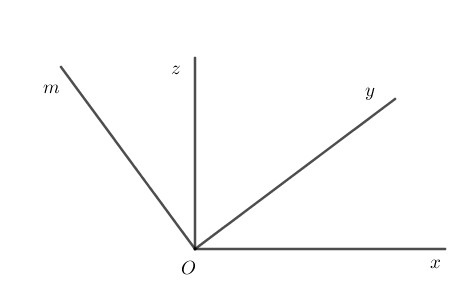
\includegraphics[width= 0.5\linewidth]{vd-30-7}
	\end{center}
	\loigiai{
		\begin{enumerate}[+,leftmargin=*]
			\i Điểm nằm trong góc $\widehat{mOn}$: $M,N,T$.
			\i Điểm không nằm trong góc $\widehat{mOn}$: $B,V,A$.
		\end{enumerate}
	}
\end{vd}
\begin{vd}
	Liệt kê các góc có trong hình vẽ sau. Em hãy đo các góc đó và so sánh các góc.
	\begin{center}
		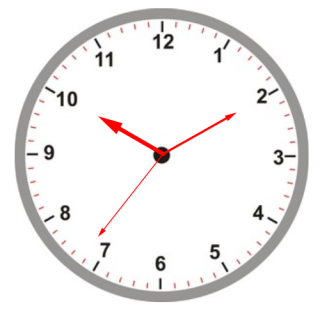
\includegraphics[width= 0.5\linewidth]{vd-30-8}
	\end{center}
	\loigiai{
		Các góc: $\widehat{zOy},\widehat{xOz},\widehat{xOy}$\\
		$\widehat{zOy}={{60}^\circ},\,\,\,\,\widehat{xOz}={{120}^\circ},\,\,\,\,\widehat{xOy}={{180}^\circ}$\\
		$\widehat{zOy}<\widehat{xOz}<\widehat{xOy}$.
	}
\end{vd}
\subsection{MỞ RỘNG KIẾN THỨC}
\subsubsection{Vẽ góc khi có số đo cho trước bằng thước đo góc}
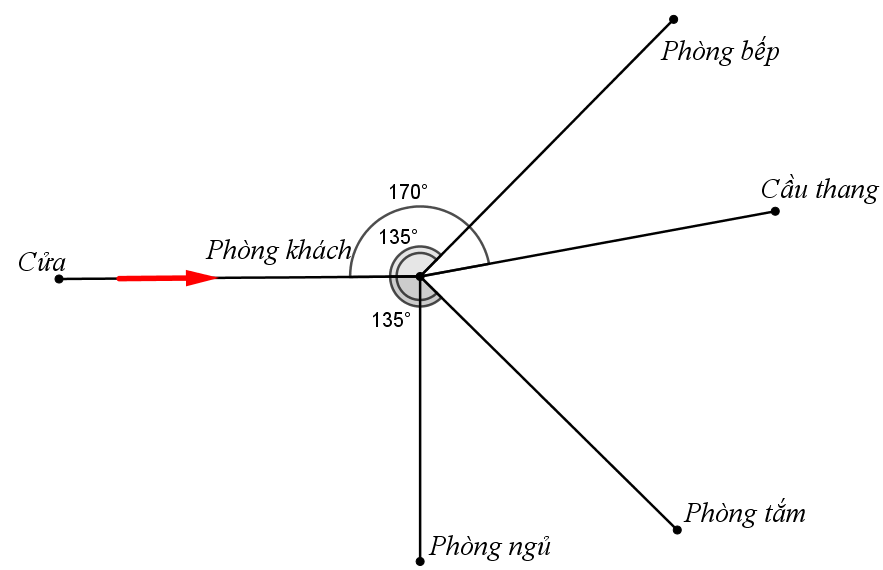
\includegraphics[width= 0.5\linewidth]{vd-30-9}
\begin{enumerate}[+,leftmargin=*]
	\i Vẽ góc $\widehat{xOy}={{m}^\circ}\left( 0<m<180 \right)$
	\begin{enumerate}[--,leftmargin=*]
		\i Vẽ tia $Ox$
		\i Đặt thước đo góc sao cho tâm thước trùng với gốc $O$ của tia $Ox$ và tia $Ox$ đi qua vạch ${{0}^\circ}$.
		\i Kẻ tia $Oy$ qua vạch ${{m}^\circ}$ của thước.
	\end{enumerate}
\end{enumerate}
\subsubsection{Công thức cộng góc}
Cho điểm $M$ nằm trong $\widehat{xOy}$. Khi đó: $\widehat{xOM}+\widehat{MOy}=\widehat{xOy}$.
\subsubsection{Công thức tính số góc tạo thành từ các tia chung gốc cho trước.}
Cho $n$ tia phân biệt chung gốc. Cứ 2 tia chung gốc tạo thành một góc. Khi đó số góc tạo bởi 2 trong $n$ tia trên là: $\dfrac{n(n-1)}{2}$ góc
\subsection{BÀI TẬP TỰ LUYỆN}
\Opensolutionfile{loigiaichung}[loigiaichuong30]
\subsubsection*{Mức độ cơ bản}
\begin{bt}
	\immini{Bài 1. Quan sát hình bên và: 
		\begin{enumerate}[a),leftmargin=*]
			\i Đọc tên các góc trong hình vẽ. Mỗi góc, hãy cho biết các đỉnh và các cạnh của nó.
			\i Xác định điểm nằm trong, nằm ngoài của mỗi góc trên.
	\end{enumerate}}{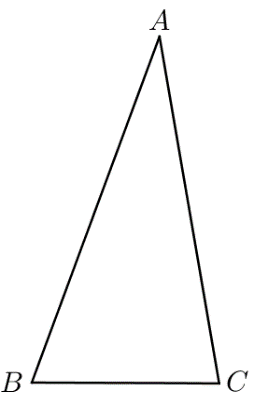
\includegraphics[width= 0.5\linewidth]{vd-30-10}}
	\begin{loigiaichuong30}
		\begin{enumerate}[a),leftmargin=*]
			\i Các góc trong hình vẽ:
			\begin{enumerate}[--,leftmargin=*]
				\i $\widehat{xOy}$: đỉnh $O$; cạnh $Ox,Oy$.
				\i $\widehat{yOz}$: đỉnh $O$; cạnh $Oy,Oz$.
				\i $\widehat{xOz}$: đỉnh $O$; cạnh $Ox,Oz$.
			\end{enumerate}
			\i Các điểm nằm trong góc $\widehat{xOy}:\,\,N,P$.
			\begin{enumerate}[--,leftmargin=*]
				\i Các điểm nằm ngoài góc $\widehat{xOy}:\,\,M,K$.
				\i Các điểm nằm trong góc $\widehat{yOz}:\,\,M$.
				\i Các điểm nằm ngoài góc $\widehat{yOz}:\,\,N,P,K$.
				\i Các điểm nằm trong góc $\widehat{xOz}:\,\,M,N,P$.
				\i Các điểm nằm ngoài góc $\widehat{xOz}:\,\,K$.
			\end{enumerate}
		\end{enumerate}
	\end{loigiaichuong30}
\end{bt}
\begin{bt}%%%%%%%%
	Viết tên các góc có đỉnh $A;M;H$ có trong hình vẽ.
	\begin{center}
		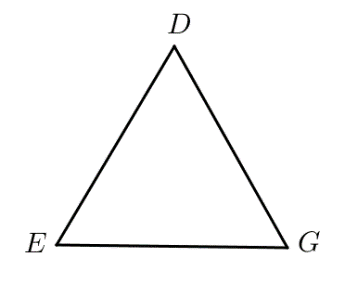
\includegraphics[width= 0.5\linewidth]{vd-30-11}
	\end{center}
	\begin{loigiaichuong30}
		Các góc có đỉnh $A:\,\,\widehat{BAH},\widehat{BAM},\widehat{BAC},\widehat{HAM},\widehat{HAC},\widehat{MAC}$.
		
		Các góc có đỉnh $M:\,\,\widehat{AMC},\widehat{AMH},\widehat{AMB}$.
		
		Các góc có đỉnh .
	\end{loigiaichuong30}
\end{bt}
\begin{bt}
	Quan sát các hình sau:
	\begin{center}
		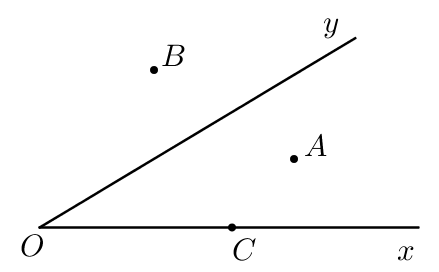
\includegraphics[width= 0.5\linewidth]{vd-30-12}
	\end{center}
	\begin{enumerate}[a),leftmargin=*]
		\i Ước lượng bằng mắt xem góc nào là góc nhọn, góc vuông, góc tù, góc bẹt.
		\i Dùng êke để kiểm tre lại kết quả của câu a.
		\i Dùng thước đo góc để tìm số đo của mỗi góc trên.
	\end{enumerate}
	\begin{loigiaichuong30}
		\begin{enumerate}[a),leftmargin=*]
			\i Góc nhọn: $\widehat{MNP}$; góc tù: $\widehat{mDn}$; góc vuông: $\widehat{ABC},\widehat{xGk},\widehat{yOz}$; góc bẹt: $\widehat{FEQ}$.
			\i Dùng êke kiểm tra lại kết quả.
			\i Dùng thước đo góc: $\widehat{MNP}={{30}^\circ},\widehat{yOz}={{90}^\circ},\widehat{ABC}={{90}^\circ},\widehat{mDn}={{135}^\circ},\widehat{FEQ}={{180}^\circ},\widehat{xGk}={{90}^\circ}$
		\end{enumerate}
	\end{loigiaichuong30}
\end{bt}
\begin{bt}
	Quan sát hìn ảnh của mặt đồng hồ, em hãy tìm hai thời điểm mà góc tạo bởi kim giờ và kim phút là:
	
	\begin{tabularx}{\textwidth}{*{2}{Z}}
		a) góc nhọn	&b) góc tù\\
		c) góc bẹt	&d) góc vuông
	\end{tabularx}
	\begin{loigiaichuong30}
		Góc tạo bởi kim giờ và kim phút là:
		\begin{enumerate}[a),leftmargin=*]
			\i góc nhọn: lúc 2 giờ, 11 giờ.
			\i góc tù: lúc 4 giờ, 5 giờ.
			\i góc bẹt: lúc 6 giờ.
			\i góc vuông: lúc 3 giờ, 9 giờ.
		\end{enumerate}
	\end{loigiaichuong30}
\end{bt}
\begin{bt}
	Em hãy nêu các hình ảnh thực tế về góc.	
	\begin{loigiaichuong30}
		Hình ảnh thực tế về góc:
		\begin{enumerate}[+,leftmargin=*]
			\i Góc tạo bởi kim phút và kim giây của đồng hồ.
			\i Góc tạo bởi cái bóng và cây cột giữa trời nắng và mặt đất.
		\end{enumerate}
	\end{loigiaichuong30}
\end{bt}
\begin{bt}
	\immini{Quan sát hình vẽ và cho biết: 
		\begin{enumerate}[a),leftmargin=*]
			\i Số góc có trong hình vẽ.
			\i Nêu tên các góc ở câu a và cho biết số đo của mỗi góc. 
	\end{enumerate}}{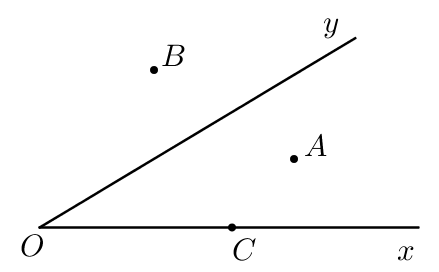
\includegraphics[width= 0.5\linewidth]{vd-30-12}}
	\begin{loigiaichuong30}
		\begin{enumerate}[a),leftmargin=*]
			\i Có 12 góc.
			\i $\widehat{ABC}={{55}^\circ};\widehat{BAC}={{80}^\circ};\widehat{ACB}={{45}^\circ};\widehat{ADB}={{110}^\circ};\widehat{BDC}={{130}^\circ};\widehat{ADC}={{120}^\circ}$
			$\widehat{CBD}={{25}^\circ},\widehat{DBA}={{20}^\circ},\widehat{BCD}={{20}^\circ},\widehat{DCA}={{25}^\circ},\widehat{BAD}={{40}^\circ},\widehat{CAD}={{40}^\circ}$
		\end{enumerate}
	\end{loigiaichuong30}
\end{bt}
\begin{bt}
	\begin{enumerate}[a),leftmargin=*]
		\i Vẽ tam giác $ABC$ bất kì. Ước lượng số đo các góc của tam giác rồi đo và cho biết tổng 3 góc trong tam giác đó là bao nhiêu?
		\i Vẽ tam giác đều $DEG$. Đo các góc của tam giác.
		\i Vẽ $\Delta MNP$ có $\widehat{M}={{90}^\circ},MP=MN$. Đo các góc $\widehat{B}$ và $\widehat{C}$.
	\end{enumerate}
	\begin{loigiaichuong30}
		\begin{enumerate}[a),leftmargin=*]
			\i Tam giác $ABC$ có:
			\begin{enumerate}[--,leftmargin=*]
				\i $\widehat{BAC}={{30}^\circ}$
				\i $\widehat{ABC}={{70}^\circ}$
				\i $\widehat{ACB}={{80}^\circ}$
				\i $\widehat{BAC}+\widehat{ABC}+\widehat{ACB}={{180}^\circ}$
			\end{enumerate}
			\i Tam giác đều $DEG$ có:
			\begin{enumerate}[--,leftmargin=*]
				\i $\widehat{D}={{60}^\circ}$
				\i $\widehat{G}={{60}^\circ}$
				\i $\widehat{E}={{60}^\circ}$
			\end{enumerate}
		\end{enumerate}
	\end{loigiaichuong30}
\end{bt}
\begin{bt}
	Tính góc tạo bởi kim giờ và kim phút của đồng hồ lúc 4 giờ, 9 giờ, 11 giờ, 6 giờ.
	\begin{loigiaichuong30}
		Góc tạo bởi kim giờ và kim phút của đồng hồ:
		\begin{enumerate}[--,leftmargin=*]
			\i lúc 4 giờ: ${{120}^\circ}$
			\i lúc 9 giờ: ${{90}^\circ}$
			\i lúc 11 giờ: ${{30}^\circ}$
			\i lúc 6 giờ: ${{180}^\circ}$
		\end{enumerate}
	\end{loigiaichuong30}
\end{bt}
\begin{bt}
	Quan sát mặt đồng hồ ở hình bên và cho biết trong các vạch chỉ số trên mặt đồng hồ, những vạch số nào nằm trong góc tạo bởi
	\immini{\begin{enumerate}[a),leftmargin=*]
			\i Kim giây và kim phút.
			\i Kim giờ và kim phút.
	\end{enumerate}}{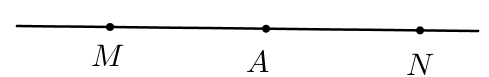
\includegraphics[width= 0.5\linewidth]{vd-30-13}}
	\begin{loigiaichuong30}
		Những vạch số nằm trong góc tạo bởi
		\begin{enumerate}[a),leftmargin=*]
			\i kim giây và kim phút: 7; 6; 5; 4; 3
			\i kim giờ và kim phút: 11; 12; 1; 1
		\end{enumerate}
	\end{loigiaichuong30}
\end{bt}
\begin{bt}%%%%%
	\immini{Quan sát hình vẽ bên
		\begin{enumerate}[a),leftmargin=*]
			\i Đọc tên các góc có trong hình vẽ.
			\i Đo và cho biết góc nhọn, góc vuông, góc tù.
			\i Viết tên các cặp góc có số đo bằng nhau.
	\end{enumerate}}{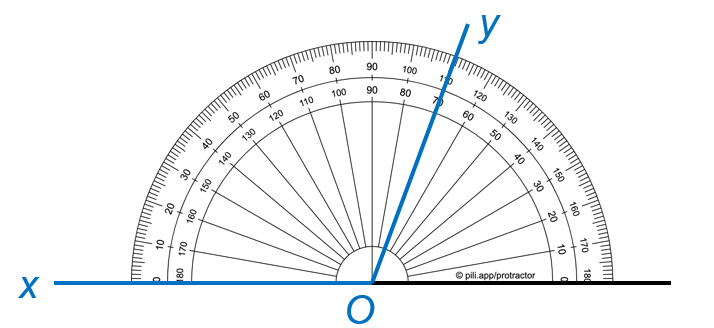
\includegraphics[width= 0.5\linewidth]{vd-30-14}}
	\begin{loigiaichuong30}
		\begin{enumerate}[a),leftmargin=*]
			\i Các góc có trong hình vẽ: $\widehat{mOz},\widehat{mOy},\widehat{mOx},\widehat{zOy},\widehat{zOx},\widehat{yOx}$
			\i Góc nhọn: $\widehat{mOz},\widehat{zOy},\widehat{yOx}$; góc vuông: $\widehat{mOn},\widehat{xOz}$; góc tù: $\widehat{xOm}$.
		\end{enumerate}
	\end{loigiaichuong30}
\end{bt}
\begin{bt}
	Điền từ thích hợp vào chỗ chấm. Đi từ cửa đến phòng khách rẽ trái theo góc ${{135}^\circ}$ thì đến \ldots 
	\begin{center}
		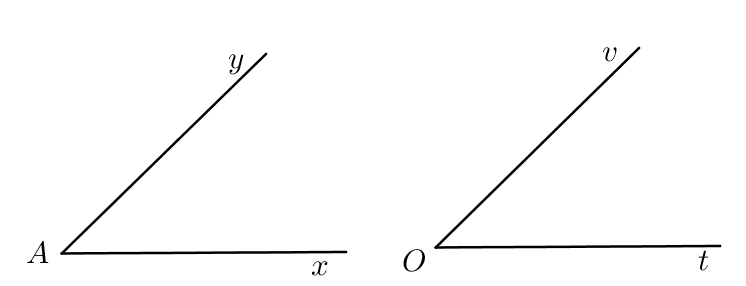
\includegraphics[width= 0.5\linewidth]{vd-30-15}
	\end{center}
	\begin{tabularx}{\textwidth}{*{4}{Y}}
	A. Phòng bếp&	B. Cầu thang&	C. Phòng tắm	&D. Phòng ngủ
	\end{tabularx}
	\begin{loigiaichuong30}
		A. Phòng bếp.
	\end{loigiaichuong30}
\end{bt}
\subsubsection{Mức độ nâng cao}
\begin{bt}
	Cho năm tia phân biệt chung gốc $Ox,Om,Oy,On,Ot$. Số góc tạo bởi hai trong năm tia là bao nhiêu
	\begin{loigiaichuong30}
		Số góc tạo bởi hai trong năm tia là:
		\begin{enumerate}[--,leftmargin=*]
			\i Số góc tạo bởi tia $Ox$ với 1 trong 4 tia còn lại là: 4 góc.
			\i Số góc tạo bởi tia $Om$ với 1 trong 3 tia còn lại (không kể $Ox$) là: 3 góc.
			\i Số góc tạo bởi tia $Oy$ với 1 trong 2 tia còn lại (không kể $Ox,Oy$) là: 2 góc.
			\i Số góc tạo bởi tia $On$ với tia $Ot$ còn lại là: 1 góc.
		\end{enumerate}
		Vậy số góc tạo thành là: $4+3+2+1=10$ góc.
	\end{loigiaichuong30}
\end{bt}
\begin{bt}
	Cho bốn tia chung gốc $Ox,Om,Oy,On$, trong đó hai tia $Oy,On$ đối nhau. Số góc tạo bởi hai trong bốn tia không kể góc bẹt là bao nhiêu?
	\begin{loigiaichuong30}
		Xét góc tạo bởi tia thứ nhất với 1 trong 3 tia còn lại có 3 góc.\\
		Xét góc tạo bởi tia thứ 2 với 1 trong 2 tia còn lại có 2 góc.\\
		Xét góc tạo bởi tia thứ 3 với 1 tia còn lại có 1 góc.\\
		Do đó, số góc tạo thành: $3+2+1=6$ góc.\\
		Vì $Oy,On$ là hai tia đối nên tạo thành 1 góc bẹt.\\
		Vậy số góc tạo bởi 2 trong 4 tia không kể góc bẹt là: $6-1=5$ góc.
	\end{loigiaichuong30}
\end{bt}
\begin{bt}
	Cho $n$ tia chung gốc, biết chúng tạo thành 21 góc. Tìm giá trị của $n$.
	\begin{loigiaichuong30}
		Số góc tạo bởi tia thứ nhất với 1 trong $n-1$ tia còn lại là $n-1$ góc.\\
		Số góc tạo bởi tia thứ hai với 1 trong $n-2$ tia còn lại là $n-2$ góc.\\
		\ldots \\
		Số góc tạo bởi tia thứ $n-1$ với tia thứ $n$ là 1 góc.\\
		Do đó, tổng số góc là: $1+2+...+n-2+n-1=n\cdot\left( n-1 \right):2$\\
		Ta có: $n\cdot\left( n-1 \right):2=21\Rightarrow n\cdot\left( n-1 \right)=42$\\
		mà $42=7\cdot6$ nên $n=7$
	\end{loigiaichuong30}
\end{bt} 
\begin{bt}
	Cho $n$ tia chung gốc $O$. Sau khi xóa một tia đi qua gốc $O$ thì số góc giảm đi 10. Tìm giá trị của $n$.
	\begin{loigiaichuong30}
		Ta có:\\
		Xóa 1 tia gốc $O$ thì số góc giảm đi 10\\
		Khi chưa xóa tia, số góc tạo bởi tia đó với $n-1$ tia còn lại là $n-1$ góc.\\
		Số góc giảm đi 10 khi xóa 1 tia nên: $n-1=10 \Rightarrow n=11$.
	\end{loigiaichuong30}
\end{bt}
\begin{bt}
	Cho $\widehat{MAN}$ là góc bẹt và tia $AT$. Biết $\widehat{MAT}-\widehat{NAT}={{8}^\circ}$. Tính $\widehat{NAT}$.
	\begin{loigiaichuong30}
		Ta có: $\widehat{MAN}$ là góc bẹt nên $\widehat{MAN}={{180}^\circ}$.\\
		$\widehat{MAT}+\widehat{NAT}=\widehat{MAN}\Rightarrow \widehat{MAT}+\widehat{NAT}={{180}^\circ}$\\
		mà  $\widehat{MAT}-\widehat{NAT}={{8}^\circ}$  nên:
		$\widehat{MAT}=\left({{180}^\circ}+{{8}^\circ}\right):2={{94}^\circ}$ \\ 
		$\widehat{NAT}=\left({{180}^\circ}-{{8}^\circ}\right):2={{86}^\circ}$ \\ 
	\end{loigiaichuong30}
\end{bt}
\Closesolutionfile{loigiaichung}
